\documentclass[10pt,a4paper]{article}
\usepackage[margin=22mm]{geometry}
\usepackage[T1]{fontenc}
\usepackage{lmodern,amsmath,amssymb,graphicx,booktabs,microtype}
\usepackage[font=small,labelfont=bf]{caption}
\usepackage[hidelinks]{hyperref}
\usepackage{fancyhdr}
\pagestyle{fancy}\fancyhf{}
\fancyhead[L]{\small Computational Mechanics Projects}
\fancyhead[R]{\small DampWatch}
\fancyfoot[C]{\thepage}
\setlength{\headheight}{14pt}
\setlength{\parindent}{0pt}\setlength{\parskip}{5pt}
\setlength{\emergencystretch}{1em}
\newcommand{\R}{\mathbb{R}}
\title{\vspace{-1.3cm}\LARGE DampWatch: Separating Physical Dissipation from Generalized-Alpha Integration Error}
\author{\small Computational Mechanics Projects\\\small Reproducible technical research note}
\date{\small 29 September 2026}
\begin{document}\maketitle\thispagestyle{fancy}

\begin{abstract}
Time integration can remove mechanical energy even when the physical damping matrix is zero. DampWatch implements the generalized-alpha method for constant linear structural systems and audits physical dissipation, applied work, and the remaining discrete energy defect. An ideal two-mass system separates low and high frequencies, and an independent matrix-exponential reference measures state error. The recorded conservative setting exhibits relative energy drift $6.63\times10^{-14}$; with high-frequency spectral radius 0.5, the low mode retains 99.9309\% of its energy while the underresolved high mode is suppressed. Refinement recovers order 1.99835. The audit distinguishes energy conservation from phase accuracy and avoids interpreting a signed budget defect as a material parameter.
\end{abstract}
\section{Introduction and mechanical system}
High-frequency numerical damping can suppress unresolved structural modes without intentionally damping resolved motion. The generalized-alpha family~\cite{chung} makes this tradeoff explicit. The research question is how physical dissipation and time-discretization effects can be reported separately without falsely equating stable energy behavior with accurate dynamics.

The unconstrained coordinates satisfy
\begin{equation}
M\ddot u+C\dot u+Ku=f(t),\qquad u(0)=u_0,\quad\dot u(0)=v_0.
\end{equation}
Matrices are real, constant, and symmetric; $M$ is positive definite and $C,K$ are positive semidefinite. Constraints must be eliminated before integration. Initial acceleration is obtained from this physical equation, not selected independently.

Using $x_{n+1-\alpha}=(1-\alpha)x_{n+1}+\alpha x_n$, the discrete equilibrium is
\begin{equation}
Ma_{n+1-\alpha_m}+Cv_{n+1-\alpha_f}+Ku_{n+1-\alpha_f}
=(1-\alpha_f)f_{n+1}+\alpha_f f_n.
\end{equation}
For prescribed asymptotic spectral radius $0\le\rho_\infty\le1$,
\begin{align}
\alpha_m&=\frac{2\rho_\infty-1}{1+\rho_\infty},&
\alpha_f&=\frac{\rho_\infty}{1+\rho_\infty},\\
\gamma&=\frac12+\alpha_f-\alpha_m,&
\beta&=\frac14(1+\alpha_f-\alpha_m)^2.
\end{align}
These are old-state weights; references using complementary alpha conventions require conversion before numerical comparison. Loads are weighted endpoint samples, not a new evaluation at an intermediate time. Smooth linear problems have second-order accuracy, while high-frequency dissipation is controlled by $\rho_\infty$.
\newpage
\section{Solution algorithm and energy accounting}
Predict $u^p=u_n+h v_n+h^2(1/2-\beta)a_n$ and $v^p=v_n+h(1-\gamma)a_n$. Solve for the new acceleration using
\begin{align}
H&=(1-\alpha_m)M+(1-\alpha_f)\gamma h C+(1-\alpha_f)\beta h^2K,\\
Ha_{n+1}&=f_{n+1-\alpha_f}-\alpha_mMa_n
-C[(1-\alpha_f)v^p+\alpha_f v_n]\nonumber\\
&\hspace{12mm}-K[(1-\alpha_f)u^p+\alpha_f u_n].
\end{align}
Then $u_{n+1}=u^p+\beta h^2a_{n+1}$ and $v_{n+1}=v^p+\gamma h a_{n+1}$. A Cholesky factorization of $H$ is reused for constant $h$. Python orchestrates the method with compiled NumPy/SciPy linear algebra. The full amplification map propagates independent basis states of $[u,hv,h^2a]$, retaining the parasitic acceleration mode.

With arithmetic endpoint averages denoted by bars, report
\begin{align}
E_n&=\tfrac12(v_n^TMv_n+u_n^TKu_n),\\
D_n&=\sum_{j<n}h\bar v_j^TC\bar v_j,\qquad
W_n=\sum_{j<n}\bar f_j^T(u_{j+1}-u_j),\\
R_n&=E_n-E_0+D_n-W_n.
\end{align}
At $\rho_\infty=1$, consistent initial acceleration yields the average-acceleration Newmark trajectory. Since $\Delta u=h\bar v$ and $\Delta v=h\bar a$, dotting mean equilibrium with $\Delta u$ gives $R_n=0$ up to roundoff. At smaller $\rho_\infty$, $R_n$ includes integration and work/dissipation quadrature errors; it is neither a monotone algorithmic energy nor physical damping.
\section{Experiment and validation}
The model is $M=\operatorname{diag}(1,0.15)$ kg and
$K=[\begin{smallmatrix}604&-600\\-600&600\end{smallmatrix}]$ N/m. Natural frequencies are 1.86490 and 67.82715 rad/s. Initial modal energies are 0.50 and 0.18 J. The 12 s free study uses $h=0.05$ s, deliberately underresolving the high mode. A forced study uses $C=0.06M+10^{-4}K$, $f=[0.8\sin(1.2t),0]^T$ N, $h=0.02$ s, and $\rho_\infty=1$.
\begin{center}\begin{tabular}{lr}\toprule
Recorded check & Value\\\midrule
Undamped relative energy drift, $\rho_\infty=1$ & $6.63\times10^{-14}$\\
Normalized forced budget defect, $\rho_\infty=1$ & $7.53\times10^{-14}$\\
Low-mode energy retention, $\rho_\infty=0.5$ & 0.9993095\\
High-frequency radius at $\omega h=10^7$, $\rho_\infty=0.5$ & 0.50001685\\
Finest observed state order & 1.99835\\\bottomrule
\end{tabular}\end{center}
An independently evaluated state-space matrix exponential~\cite{expm} supplies the damped reference at 101 common times over 2 s. At $h=0.0005$ s, the relative energy-weighted state error is 0.00595545. This quantifies accuracy rather than inferring it from stability or energy alone.
Figure~\ref{fig:results} visualizes selected recorded diagnostics.
\newpage
\begin{figure}[!ht]\centering
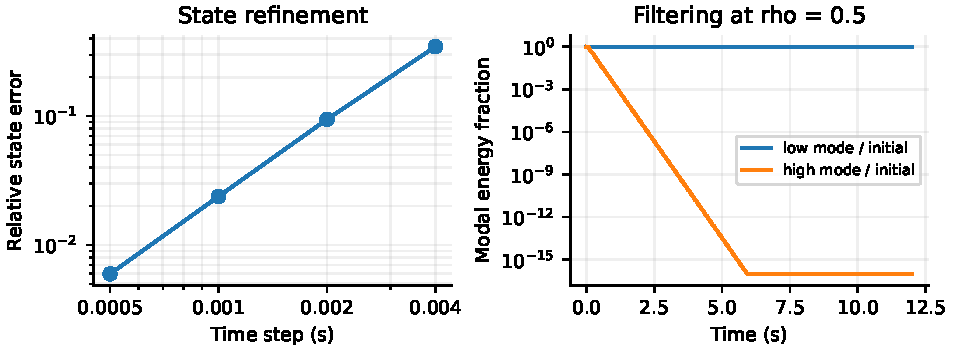
\includegraphics[width=\textwidth]{figure.pdf}
\caption{Recorded state convergence and modal-energy fractions with numerical filtering. The energy plot is clipped at $10^{-16}$ for readability; values below that level have no physical significance.}\label{fig:results}\end{figure}
\section{Discussion and limitations}
Reducing $\rho_\infty$ filters the poorly resolved attachment mode while preserving most low-mode energy. The high-mode final value below floating-point significance is not a physical measurement. The conservative parameter choice does not repair high-mode phase error. Likewise, $D_n$ approximates physical dissipation along the numerical trajectory; it is not an exact continuous-time integral.

The solver handles dense, constant linear matrices only. It has no finite-element assembly, nonlinear/contact mechanics, time-dependent matrices, algebraic constraints, adaptive steps, or restart. Storage grows with the full time history, and dense factorization costs $O(n^3)$. Abrupt loads and extreme scaling require additional validation. With rigid modes the error metric is a seminorm; the showcase stiffness is positive definite. The matrix exponential is exact in time only up to floating-point and library error.
\section{Reproducibility and conclusion}
This note documents the committed implementation at \texttt{dc5a108ad5dc} and the existing synthetic results; it does not assert new solver runs. Install from the repository root with \texttt{python -m pip install ".[dev]"}; the README gives compiler requirements and verification commands. Code, data, and this manuscript are available at \href{https://github.com/racostacme-come/dampwatch}{the project repository}. No private course material is reproduced. The manuscript was prepared with AI assistance under the project owner\textquotesingle s direction; no peer review is claimed.
Run \texttt{dampwatch --output out}. The free response, forced ledger, spectral-radius, and convergence CSVs accompany \texttt{validation.json}. The key conclusion is that damping intent, discrete energy accounting, and state accuracy are separate questions. This combination of audits exposes the tradeoff more clearly than a displacement curve alone.
\begin{thebibliography}{9}
\bibitem{chung} J. Chung and G. M. Hulbert, A time integration algorithm for structural dynamics with improved numerical dissipation: the generalized-alpha method, \emph{J. Applied Mechanics} 60(2), 371--375 (1993). \href{https://doi.org/10.1115/1.2900803}{doi:10.1115/1.2900803}.
\bibitem{expm} SciPy, \emph{scipy.linalg.expm} reference. \href{https://docs.scipy.org/doc/scipy/reference/generated/scipy.linalg.expm.html}{Matrix-exponential documentation}.
\end{thebibliography}

\end{document}
